
\documentclass{svproc}
\usepackage {graphicx, amsmath, amsfonts, algorithm, algorithmic, multirow}

\begin{document}
\mainmatter
\title{Capstone Project \\ {\large Machine Learning Engineer Nanodegree}}
\author{Dennis P. F. \\ {\small December 31, 2016}}
\institute{}
%\date{December 31, 2016}
\maketitle
\pagestyle{empty}
\section{Definition}
\subsection*{Project Overview}
This project focuses on building a learning agent for LunarLander-v2 gym environment provided by OpenAI\cite{challenge}, where the agent has to navigate a space vehicle from the starting point to the landing pad on the surface of the moon without crashing.
\subsection*{Problem Statement}
The aim of the project is to build a learning agent to navigate a space vehicle from starting point in space to the landing pad without crashing. The environment is called LunarLander-v2 which is provided by OpenAI's gym python package. At each step, the agent is provided with the current state of the space vehicle $s$ which is a 8 dimensional vector of reals $\mathbb{R}^8$ and the agent is allowed to make one of four possible actions \{ \texttt{do nothing, fire left orientation engine, fire main engine, fire right orientation engine} \} in one step. On making an action $a$, the agent gets a reward $r$ and also get to know the new state of the vehicle $s'$. If the vehicle moves from the top of the screen to reach landing pad at zero speed, it gets reward in the range $[100, 140]$. The vehicle is permitted to land outside the landing pad, but is penalized for such cases. The episode finishes if the vehicle crashes(gets additional reward of -100) or comes to rest(gets additional reward of +100) which are the end states. There is an upper limit of 1000 on the number of steps in an episode. There is no restriction on the amount of fuel used. The agent is supposed to learn a policy $\pi(s)$ that decides what action it must make at a given current state $s$ by going over the past experiences defined by the tuple $<s, a, r, s'>$. The agent is considered to have solved the environment if it gets an average reward of at least 200 over 100 consecutive trials. The objective is to minimize the number of episodes required by the agent to solve the environment. Mathematically this aim can be stated as :\\\\
Minimize i such that\\\\$\frac{\displaystyle\sum_{j=i+1}^{i+100} R_j}{100} \ge 200$\\\\
and $R_j = \displaystyle\sum_{k=1}^{N_j} r_k$; $N_j \le 1000$\\\\
where $i$ and $j$ are episode indices, $R_j$ is the total reward the agent obtained in episode $j$, $k$ is the step index in a given episode and $N_j$ is the number of steps in episode $j$. $r_k$ is the reward obtained by the agent in step $k$.
\subsection*{Scoring}
The agent's score is the number of episodes needed before it completed 100 consecutive episodes over which it got an average reward of at least 200. So an agent that learns faster with minimum number of episodes and solves is considered better than an agent that solves the problem only after learning for larger number of episodes.
\section{Analysis}
\subsection*{Data Exploration}
The state space is $\mathbb{R}^8$. The first two dimensions indicate the coordinates of the vehicle. Third and fourth dimensions indicate x and y components of the velocity of the vehicle. Fifth component specifies angle between lander pad and the vehicle base. Sixth component gives the angular velocity with respect to lander pad. Seventh and eighth dimensions indicate whether the legs of the vehicle has made ground contact or not. There are four discrete actions that the agent can make in one step : \{ \texttt{do nothing, fire left orientation engine, fire main engine, fire right orientation engine} \}.The vehicle always starts at top middle of the screen in every episode and the lander pad is always at coordinates (0,0). The episode ends when the vehicle reaches any of its end states : 1) lands on the landing pad with zero speed 2) Vehicle crashes. It is assumed that state observation made by the agent is accurate however no assumption is made as to whether the state transition is deterministic with respect to any action made by the agent.
\subsection*{Exploratory Visualization}
Following bar-charts show the mean and standard deviation of the 8 state space components in an experiment where a random action was chosen in each step per episode for 500 such episodes.\\
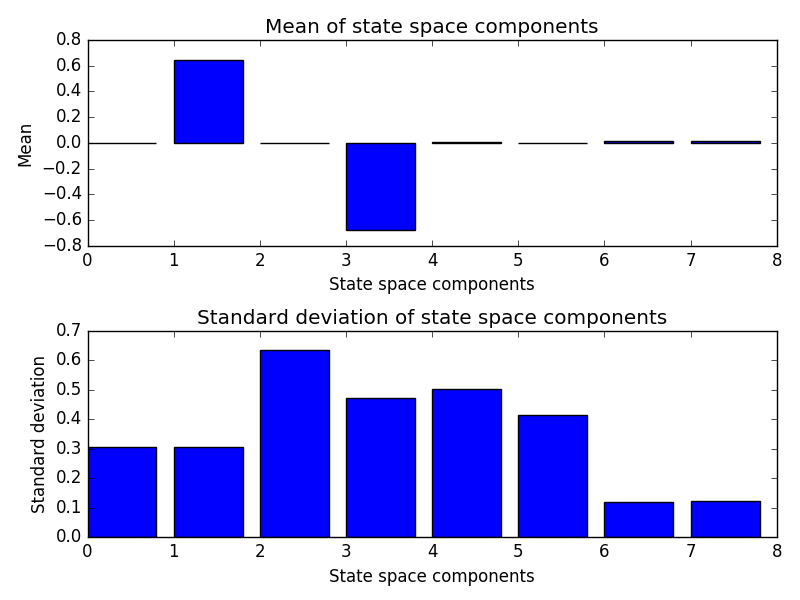
\includegraphics[width=11cm]{img/state-space}\\
The bar-charts indicate that the y coordinate(index 1) of the vehicle and y component of velocity(index 3) have their mean away from 0 while all other components have mean close to 0. Second plot indicate relatively higher standard deviation in x component of the vehicle's velocity and lower value for last two components of state space.
\subsection*{Algorithms and Techniques}
\subsection*{Benchmark}
\section{Methodology}
\subsection*{Data Processing}
\subsection*{Implementation}
\section{Results}
\section{Conclusion}
\begin{thebibliography}{}
\bibitem{challenge}
LunarLander-v2 gym environment provided by OpenAI - \texttt{https://gym.openai.com/envs/LunarLander-v2}
\end{thebibliography}

\end{document}
